\mfpicnumber{1}

\opengraphsfile{AlgebraicFunctions}

\setcounter{footnote}{0}

\label{AlgebraicFunctions}

This section serves as a watershed for functions which are combinations of polynomial, and more generally, rational functions, with the operations of radicals.  It is business of Calculus to discuss these functions in all the detail they demand so our aim in this section is to help shore up the requisite skills needed so that the reader can answer Calculus's call when the time comes.   We briefly recall the definition and some of the basic properties of radicals from Intermediate Algebra.\footnote{Although we discussed imaginary numbers in Section \ref{ComplexZeros}, we restrict our attention to real numbers in this section.  See the epilogue on page \pageref{complexepilogue} for more details.} 

\smallskip

\colorbox{ResultColor}{\bbm

\begin{defn} \label{principalnthrootdefn} Let $x$ be a real number and $n$ a natural number.\footnote{Recall this means $n=1,2,3,\ldots$.} If $n$ is odd, the \index{$n^{\textrm{th}}$ root ! principal}\index{principal $n^{\textrm{th}}$ root}\textbf{principal \boldmath $n^{\textbf{th}}$ root} of $x$, denoted $\sqrt[n]{x}$ is the unique real number satisfying $\left(\sqrt[n]{x}\right)^n = x$.  If $n$ is even, $\sqrt[n]{x}$ is defined similarly\footnote{Recall both $x=-2$ and $x=2$ satisfy $x^4=16$, but $\sqrt[4]{16} =2$, not $-2$.} provided  $x \geq 0$ and $\sqrt[n]{x} \geq 0$.  The \index{root ! index}\index{index of a root}\textbf{index} is the number $n$ and the \index{root ! radicand}\index{radicand}\textbf{radicand} is the number $x$.  For $n=2$, we write $\sqrt{x}$ instead of $\sqrt[2]{x}$.

\end{defn}

\ebm}

\smallskip

It is worth remarking that, in light of Section \ref{InverseFunctions}, we could define $f(x) = \sqrt[n]{x}$ functionally as the inverse of $g(x) = x^n$ with the stipulation that when $n$ is even, the domain of $g$ is restricted to $[0, \infty)$. From what we know about $g(x) = x^n$ from Section \ref{GraphsofPolynomials} along with Theorem \ref{inverseuniquegraph}, we can produce the graphs of $f(x) = \sqrt[n]{x}$ by reflecting the graphs of $g(x) = x^n$ across the line $y=x$.  Below are the graphs of $y=\sqrt{x}$, $y=\sqrt[4]{x}$ and $y=\sqrt[6]{x}$.  The point $(0,0)$ is indicated as a reference.  The axes are hidden so we can see the vertical steepening near $x=0$ and the horizontal flattening as $x \rightarrow \infty$.

\[ \begin{array}{ccc}

\begin{mfpic}[10]{0}{9}{0}{3}

\arrow \parafcn{0,3,0.1}{(t^2,t)}

\point[2pt]{(0,0)}

\tcaption{\scriptsize $y=\sqrt{x}$}
\end{mfpic}

&

\begin{mfpic}[10]{0}{9}{0}{3}

\arrow \parafcn{0,1.732,0.1}{(t^4,t)}

\point[2pt]{(0,0)}

\tcaption{\scriptsize $y=\sqrt[4]{x}$}

\end{mfpic}

&


\begin{mfpic}[10]{0}{9}{0}{3}

\arrow \parafcn{0,1.442,0.1}{(t^6,t)}

\point[2pt]{(0,0)}

\tcaption{\scriptsize $y=\sqrt[6]{x}$}

\end{mfpic}



\end{array}\]

The odd-indexed radical functions also follow a predictable trend - steepening near $x = 0$ and flattening as $x \rightarrow \pm \infty$.  In the exercises, you'll have a chance to graph some basic radical functions using the techniques presented in Section \ref{Transformations}.

\[ \begin{array}{ccc}

\begin{mfpic}[10]{-9}{9}{0}{3}

\arrow \reverse \arrow \parafcn{-1.587,1.587,0.1}{(t^3,t)}

\point[2pt]{(0,0)}

\tcaption{\scriptsize $y=\sqrt[3]{x}$}
\end{mfpic}

&

\begin{mfpic}[10]{-9}{9}{0}{3}

\arrow \reverse \arrow \parafcn{-1.319,1.319,0.1}{(t^5,t)}

\point[2pt]{(0,0)}

\tcaption{\scriptsize $y=\sqrt[5]{x}$}

\end{mfpic}

&


\begin{mfpic}[10]{-9}{9}{0}{3}

\arrow \reverse \arrow \parafcn{-1.219,1.219,0.1}{(t^7,t)}

\point[2pt]{(0,0)}

\tcaption{\scriptsize $y=\sqrt[7]{x}$}

\end{mfpic}



\end{array}\]


We have used all of the following properties at some point in the textbook for the case $n=2$ (the square root), but we list them here in generality for completeness.

\smallskip


\colorbox{ResultColor}{\bbm
\begin{thm}  \textbf{Properties of Radicals:} Let $x$ and $y$ be real numbers and $m$ and $n$ be natural numbers.  If $\sqrt[n]{x}$,  $\sqrt[n]{y}$ are real numbers, then \index{radical ! properties of}

\label{radicalprops}

\begin{itemize}

\item  \textbf{Product Rule:}  $\sqrt[n]{xy} = \sqrt[n]{x} \, \sqrt[n]{y}$ \index{product rule ! for radicals}

\item  \textbf{Powers of Radicals:} $\sqrt[n]{x^m} = \left(\sqrt[n]{x}\right)^m$ \index{power rule ! for radicals}

\item  \textbf{Quotient Rule:}  $\sqrt[n]{\dfrac{x}{y}} = \dfrac{\sqrt[n]{x}}{\sqrt[n]{y}}$, provided $y \neq 0$. \index{quotient rule ! for radicals}

\item  If $n$ is odd, $\sqrt[n]{x^n} = x$; if $n$ is even, $\sqrt[n]{x^n} = |x|$.

\end{itemize}

\end{thm}

\ebm}

\medskip

The proof of Theorem \ref{radicalprops} is based on the definition of the principal roots and properties of exponents. To establish the product rule, consider the following.  If $n$ is odd, then by definition $\sqrt[n]{xy}$ is the unique real number such that $(\sqrt[n]{xy})^{n} = xy$.  Given that $\left( \sqrt[n]{x} \, \sqrt[n]{y}\right)^n = \left(\sqrt[n]{x}\right)^n \left(\sqrt[n]{y}\right)^n = xy$, it must be the case that $\sqrt[n]{xy} = \sqrt[n]{x} \, \sqrt[n]{y}$. If $n$ is even, then $\sqrt[n]{xy}$ is the unique non-negative real number such that $(\sqrt[n]{xy})^{n} = xy$.  Also note that since $n$ is even, $\sqrt[n]{x}$ and $\sqrt[n]{y}$ are also non-negative and hence so is $\sqrt[n]{x}\sqrt[n]{y}$.  Proceeding as above, we find that $\sqrt[n]{xy} = \sqrt[n]{x} \, \sqrt[n]{y}$.  The quotient rule is proved similarly and is left as an exercise.  The power rule results from repeated application of the product rule, so long as $\sqrt[n]{x}$ is a real number to start with.\footnote{Otherwise we'd run into the same paradox we did in Section \ref{ComplexZeros}.}  The last property is an application of the power rule when $n$ is odd, and the occurrence of the absolute value when $n$ is even is due to the requirement that  $\sqrt[n]{x} \geq 0$ in Definition \ref{principalnthrootdefn}. For instance, $\sqrt[4]{(-2)^4} = \sqrt[4]{16}= 2 =  |-2|$, not $-2$.   It's this last property which makes compositions of roots and powers delicate.  This is especially true when we use exponential notation for radicals.  Recall the following definition.

\smallskip

\colorbox{ResultColor}{\bbm

\begin{defn}  \label{rationalexponentdefn} Let $x$ be a real number,  $m$ an integer\footnote{Recall this means $m = 0, \pm 1, \pm 2, \ldots$} and $n$ a natural number. \index{rational exponent}

\begin{itemize}

\item  $x^{\frac{1}{n}} = \sqrt[n]{x}$ and is defined whenever $\sqrt[n]{x}$ is defined.

\item  $x^{\frac{m}{n}}  = \left(\sqrt[n]{x}\right)^m = \sqrt[n]{x^m}$, whenever $\left(\sqrt[n]{x}\right)^{m}$ is defined.

\end{itemize}
\end{defn}

\ebm}

\smallskip

The rational exponents defined in Definition \ref{rationalexponentdefn} behave very similarly to the usual integer exponents from Elementary Algebra with one critical exception.  Consider the expression $\left(x^{2/3}\right)^{3/2}$.  Applying the usual laws of exponents, we'd be tempted to simplify this as $\left(x^{2/3}\right)^{3/2} = x^{\frac{2}{3} \cdot \frac{3}{2}} = x^{1} = x$.  However, if we substitute $x=-1$ and apply Definition \ref{rationalexponentdefn}, we find $(-1)^{2/3} = \left(\sqrt[3]{-1}\right)^2 = (-1)^2 = 1$ so that $\left((-1)^{2/3}\right)^{3/2} = 1^{3/2} = \left(\sqrt{1}\right)^3 = 1^3 = 1$.  We see in this case that $\left(x^{2/3}\right)^{3/2} \neq x$.  If we take the time to rewrite $\left(x^{2/3}\right)^{3/2}$ with radicals, we see 

\[ \left(x^{2/3}\right)^{3/2} = \left(\left(\sqrt[3]{x}\right)^2\right)^{3/2} =  \left(\sqrt{\left(\sqrt[3]{x}\right)^2}\right)^3 =\left(\left|\sqrt[3]{x}\right|\right)^3 = \left| \left(\sqrt[3]{x}\right)^3  \right| = |x|\]

In the play-by-play analysis, we see that when we canceled the $2$'s in multiplying $\frac{2}{3} \cdot \frac{3}{2}$, we were, in fact, attempting to cancel a square with a square root.  The fact that $\sqrt{x^2} = |x|$ and not simply $x$ is the root\footnote{Did you like that pun?} of the trouble.  It may amuse the reader to know that  $\left(x^{3/2}\right)^{2/3} = x$, and this verification is left as an exercise.  The moral of the story is that when simplifying fractional exponents, it's usually best to rewrite them as radicals.\footnote{In most other cases, though, rational exponents are preferred.}   The last major property we will state, and leave to Calculus to prove, is that radical functions are continuous on their domains, so the Intermediate Value Theorem, Theorem \ref{IVT}, applies.  This means that if we take combinations of radical functions with polynomial and rational functions to form what the authors consider \index{function ! algebraic} the \textbf{algebraic functions},\footnote{As mentioned in Section \ref{AbsoluteValueFunctions}, $f(x) = \sqrt{x^2}=|x|$ so that absolute value is also considered an algebraic function.} we can make sign diagrams using the procedure set forth in Section \ref{RationalGraphs}.  

\medskip

\phantomsection
\label{algebraicsigndiagram}

\colorbox{ResultColor}{\bbm

\smallskip

\centerline{\textbf{Steps for Constructing a Sign Diagram for an Algebraic Function}} \index{sign diagram ! algebraic function}

\smallskip

\hspace{.17in} Suppose $f$ is an algebraic function.

\begin{enumerate}

\item  Place any values excluded from the domain of  $f$ on the number line with an `\textinterrobang' above them.

\item  Find the zeros of $f$ and place them on the number line with the number $0$ above them.

\item  Choose a test value in each of the intervals determined in steps 1 and 2.

\item  Determine the sign of $f(x)$ for each test value in step 3, and write that sign above the corresponding interval.

\end{enumerate}

\ebm}

\medskip 

Our next example reviews quite a bit of Intermediate Algebra and demonstrates some of the new features of these graphs.

\begin{ex}  For the following functions, state their domains and create sign diagrams.  Check your answer graphically using your calculator. 

\begin{multicols}{2}
\begin{enumerate}

\item  $f(x) = 3x \sqrt[3]{2-x}$

\item  $g(x) = \sqrt{2-\sqrt[4]{x+3}}$

\setcounter{HW}{\value{enumi}}
\end{enumerate}
\end{multicols}

\begin{multicols}{2}
\begin{enumerate}
\setcounter{enumi}{\value{HW}}

\item  $h(x) = \sqrt[3]{\dfrac{8x}{x+1}}$

\item  $k(x) = \dfrac{2x}{\sqrt{x^2 - 1}}$

\setcounter{HW}{\value{enumi}}
\end{enumerate}
\end{multicols}


{\bf Solution.}

\begin{enumerate}

\item  As far as domain is concerned, $f(x)$ has no denominators and no even roots, which means its domain is $(-\infty, \infty)$.  To create the sign diagram, we find the zeros of $f$.  

\[ \begin{array}{rclr}

f(x) & = & 0 & \\

3x \sqrt[3]{2-x} & = & 0 \\

3x = 0 & \mbox{or} & \sqrt[3]{2-x} = 0 & \\

x = 0 & \mbox{or} & \left(\sqrt[3]{2-x}\right)^3 = 0^3 & \\

x = 0 & \mbox{or} & 2-x = 0 & \\

x = 0 & \mbox{or} & x=2 & \\

\end{array}\]

The zeros $0$ and $2$ divide the real number line into three test intervals.  The sign diagram and accompanying graph are below.  Note that the intervals on which $f$ is $(+)$ correspond to where the graph of $f$ is above the $x$-axis, and where the graph of $f$ is below the $x$-axis we have that $f$ is $(-)$.  The calculator suggests something mysterious happens near $x=2$.  Zooming in shows the graph becomes nearly vertical there.  You'll have to wait until Calculus to fully understand this phenomenon.

\begin{tabular}{m{2in}cc}

\begin{mfpic}[10]{-5}{5}{-1}{2}

\arrow \reverse \arrow \polyline{(-5,0),(5,0)}

\xmarks{-2,2}

\tlabel[cc](-3.5,1){$(-)$}

\tlabel[cc](-2,-1){$0$}

\tlabel[cc](-2,1){$0$}

\tlabel[cc](0,1){$(+)$}

\tlabel[cc](2,-1){$2$}

\tlabel[cc](2,1){$0$}

\tlabel[cc](3.5,1){$(-)$}

\end{mfpic}

& 

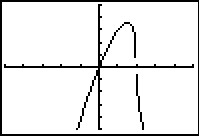
\includegraphics[width=1.5in]{./FurtherGraphics/Algebraic01.jpg}

&

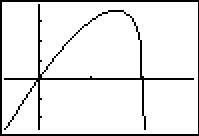
\includegraphics[width=1.5in]{./FurtherGraphics/Algebraic02.jpg} \\

& $y=f(x)$ & $y=f(x)$ near $x=2$.

\end{tabular}

\item In $g(x) = \sqrt{2-\sqrt[4]{x+3}}$, we have two radicals both of which are even indexed.  To satisfy $\sqrt[4]{x+3}$, we require $x+3 \geq 0$ or $x \geq -3$.  To satisfy $ \sqrt{2-\sqrt[4]{x+3}}$, we need $2-\sqrt[4]{x+3} \geq 0$.  While it may be tempting to write this as $2 \geq \sqrt[4]{x+3}$ and take both sides to the fourth power, there are times when this technique will produce erroneous results.\footnote{For instance, $-2 \geq \sqrt[4]{x+3}$, which has no solution or  $-2 \leq \sqrt[4]{x+3}$ whose solution is $[-3,\infty)$.}  Instead, we solve $2-\sqrt[4]{x+3} \geq 0$ using a sign diagram.  If we let $r(x) = 2-\sqrt[4]{x+3}$, we know $x \geq -3$, so we  concern ourselves with only this portion of the number line.  To find the zeros of $r$ we set $r(x) =0$ and solve  $2-\sqrt[4]{x+3}=0$.  We get $\sqrt[4]{x+3} = 2$ so that $\left(\sqrt[4]{x+3}\right)^4 = 2^4$ from which we obtain $x+3 = 16$ or $x=13$.  Since we raised both sides of an equation to an even power, we need to check to see if $x=13$ is an extraneous solution.\footnote{Recall, this means we have produced a candidate which doesn't satisfy the original equation.  Do you remember how raising both sides of an equation to an even power could cause this?}  We find $x=13$ does check since $2-\sqrt[4]{x+3} = 2 - \sqrt[4]{13+3} = 2 - \sqrt[4]{16} = 2 - 2 = 0$. Below is our sign diagram for $r$.



\begin{center}

\begin{mfpic}[10]{0}{8}{-2}{2}

\arrow \polyline{(0,0), (8,0)}

\xmarks{0,4}

\tlabel[cc](0,-1){$-3 \hspace{7pt}$}

\tlabel[cc](2,1){$(+)$}

\tlabel[cc](4,-1){$13$}

\tlabel[cc](4,1){$0$}

\tlabel[cc](6,1){$(-)$}

\end{mfpic}

\end{center}

We find $2-\sqrt[4]{x+3} \geq 0$ on $[-3,13]$ so this is the domain of $g$.  To find a sign diagram for $g$, we look for the zeros of $g$.  Setting $g(x) = 0$ is equivalent to $\sqrt{2-\sqrt[4]{x+3}}=0$.  After squaring both sides, we get $2-\sqrt[4]{x+3} = 0$, whose solution we have found to be $x=13$.   Since we squared both sides, we double check and find $g(13)$ is, in fact, $0$. Our sign diagram and graph of $g$ are below.  Since the domain of $g$ is $[-3,13]$, what we have below is not just a \textit{portion} of the graph of $g$, but the \textit{complete} graph.  It is always above or on the $x$-axis, which verifies our sign diagram.

\begin{tabular}{m{2.5in}c}

\begin{mfpic}[10]{0}{4}{-2}{2}

\polyline{(0,0), (4,0)}

\xmarks{0,4}

\tlabel[cc](0,-1){$-3 \hspace{7pt}$}

\tlabel[cc](2,1){$(+)$}

\tlabel[cc](4,-1){$13$}

\end{mfpic}

&

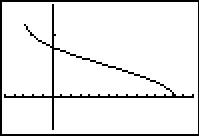
\includegraphics[width=2in]{./FurtherGraphics/Algebraic03.jpg} \\

& The complete graph of $y=g(x)$. \\

\end{tabular}

\item  The radical in $h(x)$ is odd, so our only concern is the denominator.  Setting $x+1=0$ gives $x=-1$, so our domain is $(-\infty, -1) \cup (-1, \infty)$.  To find the zeros of $h$, we set $h(x) = 0$. 
To solve $\sqrt[3]{\frac{8x}{x+1}} = 0$, we cube both sides to get $\frac{8x}{x+1} = 0$.  We get $8x=0$, or $x=0$. Below is the resulting sign diagram and corresponding graph. From the graph, it appears as though $x=-1$ is a vertical asymptote.  Carrying out an analysis as $x \rightarrow -1$ as in Section \ref{RationalGraphs} confirms this.  (We leave the details to the reader.)  Near $x=0$, we have a situation similar to $x=2$ in the graph of $f$ in number 1 above.  Finally, it appears as if the graph of $h$ has a horizontal asymptote $y=2$.  Using techniques from Section \ref{RationalGraphs}, we find as $x \rightarrow \pm \infty$, $\frac{8x}{x+1} \rightarrow 8$.  From this, it is hardly surprising that as $x \rightarrow \pm \infty$, $h(x) = \sqrt[3]{\frac{8x}{x+1}} \approx  \sqrt[3]{8} =2$.

\begin{tabular}{m{2.5in}c}

\begin{mfpic}[10]{-5}{5}{-1}{2}

\arrow \reverse \arrow \polyline{(-5,0),(5,0)}

\xmarks{-2,2}

\tlabel[cc](-3.5,1){$(+)$}

\tlabel[cc](-2,-1){$-1 \hspace{7pt}$}

\tlabel[cc](-2,1){\textinterrobang}

\tlabel[cc](0,1){$(-)$}

\tlabel[cc](2,-1){$0$}

\tlabel[cc](2,1){$0$}

\tlabel[cc](3.5,1){$(+)$}

\end{mfpic}

&

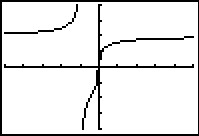
\includegraphics[width=2in]{./FurtherGraphics/Algebraic04.jpg} \\

& $y=h(x)$ \\

\end{tabular}

\item  To find the domain of $k$, we have both an even root and a denominator to concern ourselves with.  To satisfy the square root, $x^2 - 1 \geq 0$.  Setting $r(x) = x^2-1$, we find the zeros of $r$ to be $x = \pm 1$, and we find the sign diagram of $r$ to be


\begin{center}

\begin{mfpic}[10]{-5}{5}{-1}{2}

\arrow \reverse \arrow \polyline{(-5,0),(5,0)}

\xmarks{-2,2}

\tlabel[cc](-3.5,1){$(+)$}

\tlabel[cc](-2,-1){$-1 \hspace{7pt}$}

\tlabel[cc](-2,1){0}

\tlabel[cc](0,1){$(-)$}

\tlabel[cc](2,-1){$1$}

\tlabel[cc](2,1){$0$}

\tlabel[cc](3.5,1){$(+)$}

\end{mfpic}

\end{center}

We find $x^2 - 1 \geq 0$ for $(-\infty, -1] \cup [1, \infty)$.  To keep the denominator of $k(x)$ away from zero, we set $\sqrt{x^2-1} = 0$. We leave it to the reader to verify the solutions are $x = \pm 1$, both of which must be excluded from the domain.    Hence, the domain of $k$ is $(-\infty, -1) \cup (1,\infty)$.  To build the sign diagram for $k$, we need the zeros of $k$.  Setting $k(x) = 0$ results in $\frac{2x}{\sqrt{x^2 - 1}}= 0$.  We get $2x =0$ or $x=0$.  However, $x=0$ isn't in the domain of $k$, which means $k$ has no zeros.  We construct our sign diagram on the domain of $k$ below alongside the graph of $k$. It appears that the graph of $k$ has two vertical asymptotes, one at $x=-1$ and one at $x=1$.   The gap in the graph between the asymptotes is because of the gap in the domain of $k$. Concerning end behavior, there appear to be two horizontal asymptotes, $y = 2$ and $y=-2$.  To see why this is the case, we think of $x\rightarrow \pm \infty$.   The radicand of the denominator $x^2 - 1 \approx x^2$, and as such, $k(x) = \frac{2x}{\sqrt{x^2 - 1}} \approx \frac{2x}{\sqrt{x^2}} = \frac{2x}{|x|}$.  As $x \rightarrow \infty$, we have $|x| = x$ so $k(x) \approx \frac{2x}{x} = 2$.  On the other hand, as $x \rightarrow -\infty$, $|x| = -x$, and as such $k(x) \approx \frac{2x}{-x} = -2$. Finally, it appears as though the graph of $k$ passes the Horizontal Line Test which means $k$ is one to one and $k^{-1}$ exists.  Computing $k^{-1}$ is left as an exercise.

\begin{tabular}{m{2.5in}c}

\begin{mfpic}[10]{-5}{5}{-1}{2}

\arrow  \polyline{(-2,0),(-5,0)}

\arrow  \polyline{(2,0),(5,0)}

\xmarks{-2,2}

\tlabel[cc](-3.5,1){$(-)$}

\tlabel[cc](-2,-1){$-1 \hspace{7pt}$}

\tlabel[cc](-2,1){\textinterrobang}

\tlabel[cc](2,-1){$1$}

\tlabel[cc](2,1){\textinterrobang}

\tlabel[cc](3.5,1){$(+)$}

\end{mfpic}

&

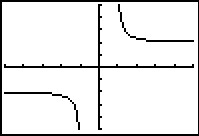
\includegraphics[width=2in]{./FurtherGraphics/Algebraic05.jpg} \\

& $y = k(x)$ \\

\end{tabular}

\qed
\end{enumerate}

\end{ex}

As the previous example illustrates, the graphs of general algebraic functions can have features we've seen before, like vertical and horizontal asymptotes, but they can occur in new and exciting ways. For example, $k(x) = \frac{2x}{\sqrt{x^{2} - 1}}$ had two distinct horizontal asymptotes.  You'll recall that rational functions could have at most one horizontal asymptote.  Also some new characteristics like `unusual steepness'\footnote{The proper Calculus term for this is `vertical tangent', but for now we'll be okay calling it `unusual steepness'.} and cusps\footnote{See page \pageref{cusppicture} for the first reference to this feature.} can appear in the graphs of arbitrary algebraic functions.   Our next example first demonstrates how we can use sign diagrams to solve nonlinear inequalities. (Don't panic.  The technique is very similar to the ones used in Chapters \ref{LinearQuadratic}, \ref{Polynomials} and \ref{Rationals}.)  We then check our answers graphically with a calculator and see some of the new graphical features of the functions in this extended family.

\begin{ex}  Solve the following inequalities.  Check your answers graphically with a calculator.

\begin{multicols}{2}
\begin{enumerate}

\item $x^{2/3} < x^{4/3} - 6$

\item  $3 (2-x)^{1/3} \leq x (2-x)^{-2/3}$

\end{enumerate}
\end{multicols}

{\bf Solution.}  

\begin{enumerate}

\item  To solve $x^{2/3} < x^{4/3} - 6$, we get $0$ on one side and attempt to solve $x^{4/3} - x^{2/3} - 6 > 0$.  We set $r(x) = x^{4/3} - x^{2/3} - 6$ and note that since the denominators in the exponents are $3$, they correspond to cube roots, which means the domain of $r$ is $(-\infty, \infty)$. To find the zeros for the sign diagram, we set $r(x) = 0$ and attempt to solve $x^{4/3} - x^{2/3} - 6 = 0$.  At this point, it may be unclear how to proceed.  We could always try as a last resort converting back to radical notation,  but in this case we can take a cue from Example \ref{usubex}.  Since there are three terms, and the exponent on one of the variable terms, $x^{4/3}$, is exactly twice that of the other, $x^{2/3}$, we have ourselves a `quadratic in disguise' and we can rewrite  $ x^{4/3} - x^{2/3} - 6 = 0$ as $\left(x^{2/3}\right)^2 - x^{2/3} - 6=0$.  If we let $u = x^{2/3}$, then in terms of $u$, we get $u^2 - u - 6 = 0$.  Solving for $u$, we obtain $u = -2$ or $u = 3$.  Replacing $x^{2/3}$ back in for $u$, we get $x^{2/3} = -2$ or $x^{2/3} = 3$.  To avoid the trouble we encountered in the discussion following Definition \ref{rationalexponentdefn}, we now convert back to radical notation.  By interpreting $x^{2/3}$ as $\sqrt[3]{x^2}$ we have $\sqrt[3]{x^2} = -2$ or $\sqrt[3]{x^2}= 3$.  Cubing both sides of these equations results in $x^2 = -8$, which admits no real solution, or $x^2 = 27$, which gives $x = \pm 3 \sqrt{3}$.  We construct a sign diagram and find $x^{4/3} - x^{2/3} - 6 > 0$ on $\left(-\infty, -3 \sqrt{3}\right)\cup \left(3 \sqrt{3}, \infty\right)$.  To check our answer graphically, we set $f(x) = x^{2/3}$ and $g(x) = x^{4/3}-6$.  The solution to  $x^{2/3} < x^{4/3} - 6$ corresponds to the inequality $f(x) < g(x)$, which means we are looking for the $x$ values for which the graph of $f$ is below the graph of $g$.  Using the `Intersect' command we confirm\footnote{Or at least confirm to several decimal places} that the graphs cross at $x= \pm 3\sqrt{3}$.  We see that the graph of $f$ is below the graph of $g$ (the thicker curve) on $\left(-\infty, -3 \sqrt{3}\right)\cup \left(3 \sqrt{3}, \infty\right)$.

\begin{center}

\begin{tabular}{m{2.5in}c}

\begin{mfpic}[10]{-5}{5}{-1}{2}

\arrow \reverse \arrow \polyline{(-5,0),(5,0)}

\xmarks{-2,2}

\tlabel[cc](-3.5,1){$(+)$}

\tlabel[cc](-2,-1){$-3 \sqrt{3} \hspace{7pt}$}

\tlabel[cc](-2,1){$0$}

\tlabel[cc](0,1){$(-)$}

\tlabel[cc](2,-1){$3 \sqrt{3}$}

\tlabel[cc](2,1){$0$}

\tlabel[cc](3.5,1){$(+)$}

\end{mfpic}

&

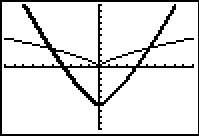
\includegraphics[width=2in]{./FurtherGraphics/Algebraic06.jpg} \\

& $y = f(x)$ and \boldmath $y = g(x)$ \\

\end{tabular}

\end{center}

As a point of interest, if we take a closer look at the graphs of $f$ and $g$  near $x=0$ with the axes off, we see that despite the fact they both involve cube roots, they exhibit different behavior near $x=0$.  The graph of $f$ has a sharp turn, or cusp, while $g$ does not.\footnote{Again, we introduced this feature on page \pageref{cusppicture} as a feature which makes the graph of a function `not smooth'.}

\begin{center}

\begin{tabular}{cc}

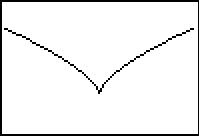
\includegraphics[width=2in]{./FurtherGraphics/Algebraic07.jpg} & 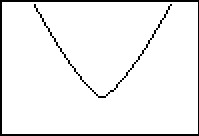
\includegraphics[width=2in]{./FurtherGraphics/Algebraic08.jpg} \\

$y=f(x)$ near $x=0$ & $y=g(x)$ near $x=0$ \\

\end{tabular}

\end{center}

\item  To solve $3 (2-x)^{1/3} \leq x (2-x)^{-2/3}$, we gather all the nonzero terms on one side and obtain $3 (2-x)^{1/3} - x (2-x)^{-2/3} \leq 0$. We set $r(x) = 3 (2-x)^{1/3} - x (2-x)^{-2/3}$.  As in number 1, the denominators of the rational exponents are odd, which means there are no domain concerns there.  However, the negative exponent on the second term indicates a denominator.  Rewriting $r(x)$ with positive exponents, we obtain \[r(x) =  3 (2-x)^{1/3} - \frac{x}{(2-x)^{2/3}}\]  Setting the denominator equal to zero we get $(2-x)^{2/3} = 0$, or $\sqrt[3]{(2-x)^2} = 0$.  After cubing both sides, and subsequently taking square roots, we get $2-x=0$, or $x=2$.  Hence, the domain of $r$ is $(-\infty, 2) \cup (2, \infty)$. To find the zeros of $r$, we set $r(x) = 0$.  There are two school of thought on how to proceed and we demonstrate both.

\begin{itemize}

\item  \textit{Factoring Approach.}  From $r(x) = 3 (2-x)^{1/3} - x (2-x)^{-2/3}$, we note that the quantity $(2-x)$ is common to both terms.  When we factor out common factors, we factor out the quantity with the \textit{smaller} exponent.  In this case, since $-\frac{2}{3} < \frac{1}{3}$, we factor $(2-x)^{-2/3}$ from both quantities.  While it may seem odd to do so, we need to factor $(2-x)^{-2/3}$ \textit{from} $(2-x)^{1/3}$, which results in subtracting the exponent $-\frac{2}{3}$ from $\frac{1}{3}$.  We proceed using the usual properties of exponents.\footnote{And we exercise special care when reducing the $\frac{3}{3}$ power to $1$.}

\[ \begin{array}{rclr}

r(x)  & = & 3 (2-x)^{1/3} - x (2-x)^{-2/3} & \\ [3pt]
      & = & (2-x)^{-2/3} \left[ 3 (2-x)^{\frac{1}{3} - \left(-\frac{2}{3}\right)} - x\right] & \\ [6pt]
      & = & (2-x)^{-2/3}\left[3(2-x)^{3/3} - x\right] & \\ [3pt]
      & = & (2-x)^{-2/3}\left[3(2-x)^{1} - x\right] & \mbox{since $\sqrt[3]{u^3} = \left(\sqrt[3]{u}\right)^{3} = u$} \\ [3pt]
      & = & (2-x)^{-2/3}\left(6-4x\right) & \\ [3pt]
      & = & (2-x)^{-2/3}\left(6-4x\right) & \\
      
\end{array}\]

To solve $r(x) = 0$, we set $(2-x)^{-2/3}\left(6-4x\right) = 0$, or $\frac{6-4x}{(2-x)^{2/3}} = 0$.  We have $6-4x = 0$ or $x = \frac{3}{2}$.

\pagebreak 

\item \textit{Common Denominator Approach.}  We rewrite 

\[ \begin{array}{rclr}

r(x)  & = & 3 (2-x)^{1/3} - x (2-x)^{-2/3} & \\ [3pt]
      & = & 3 (2-x)^{1/3} - \dfrac{x}{(2-x)^{2/3}} & \\ [10pt]
      & = & \dfrac{3 (2-x)^{1/3}(2-x)^{2/3}}{(2-x)^{2/3}} - \dfrac{x}{(2-x)^{2/3}} & \mbox{common denominator} \\ [10pt]
      & = & \dfrac{3 (2-x)^{\frac{1}{3} + \frac{2}{3}}}{(2-x)^{2/3}} - \dfrac{x}{(2-x)^{2/3}} &  \\ [10pt]
      & = & \dfrac{3 (2-x)^{3/3}}{(2-x)^{2/3}} - \dfrac{x}{(2-x)^{2/3}} & \\ [10pt]
      & = & \dfrac{3 (2-x)^1}{(2-x)^{2/3}} - \dfrac{x}{(2-x)^{2/3}} & \mbox{since $\sqrt[3]{u^3} = \left(\sqrt[3]{u}\right)^{3} = u$} \\ [10pt]
      & = & \dfrac{3 (2-x) - x}{(2-x)^{2/3}} & \\ [10pt]
      & = & \dfrac{6-4x}{(2-x)^{2/3}} & \\

       
\end{array}\]


As before, when we set $r(x) = 0$ we obtain $x = \frac{3}{2}$.


\end{itemize}

We now create our sign diagram and find  $3 (2-x)^{1/3} - x (2-x)^{-2/3} \leq 0$ on $\left[\frac{3}{2},2\right) \cup (2, \infty)$.  To check this graphically, we set $f(x)=3 (2-x)^{1/3}$ and $g(x) = x (2-x)^{-2/3}$ (the thicker curve). We confirm that the graphs intersect at $x=\frac{3}{2}$ and the graph of $f$ is below the graph of $g$ for $x \geq \frac{3}{2}$, with the exception of $x=2$ where it appears the graph of $g$ has a vertical asymptote. 

\begin{center}

\begin{tabular}{m{2.5in}c}

\begin{mfpic}[10]{-5}{5}{-1}{2}

\arrow \reverse \arrow \polyline{(-5,0),(5,0)}

\xmarks{-2,2}

\tlabel[cc](-3.5,1){$(+)$}

\tlabel[cc](-2,-1.25){$\frac{3}{2}$}

\tlabel[cc](-2,1){$0$}

\tlabel[cc](0,1){$(-)$}

\tlabel[cc](2,-1){$2$}

\tlabel[cc](2,1){\textinterrobang}

\tlabel[cc](3.5,1){$(-)$}

\end{mfpic}

&

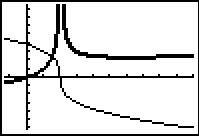
\includegraphics[width=2in]{./FurtherGraphics/Algebraic09.jpg} \\

& $y = f(x)$ and \boldmath $y = g(x)$ \\

\end{tabular}

\end{center}

\end{enumerate}

\vspace{-.30in} \qed

\end{ex}

One application of algebraic functions was given in Example \ref{distancefunctionex} in Section \ref{CartesianPlane}.  Our last example is a more sophisticated application of distance.

\begin{ex} \label{SasquatchCable} Carl wishes to get high speed internet service installed in his remote Sasquatch observation post located $30$ miles from Route $117$. The nearest junction box is located $50$ miles downroad from the post, as indicated in the diagram below.  Suppose it costs $\$ 15$ per mile to run cable along the road and $\$ 20$ per mile to run cable off of the road.

\begin{center}
\begin{mfpic}[15]{-1}{15}{-1}{9}

\xmarks{0, 4}

\arrow \reverse \arrow \polyline{(0,8.75),(0,0.25)}

\arrow \reverse \arrow \polyline{(0.25,0),(3.75,0)}

\arrow \reverse \arrow \polyline{(4.25,0),(9.75,0)}

\arrow \reverse \arrow \polyline{(0,-1),(10,-1)}

\dashed \polyline{(4,0),(0,9)}

\point[3pt]{(0,9), (10,0)}

\tlabel[cc](1.25,9){\scriptsize Outpost}

\tlabel[cc](12,0){\scriptsize Junction Box}

\tlabel[cc](7,0.5){$x$}

\tlabel[cc](2,0.5){$y$}

\tlabel[cc](3,4.5){$z$}

\tlabel[cc](5,-.5){\scriptsize Route $117$}

\tlabel[cc](5,-2){\scriptsize $50$ miles}

\tlabel[cc](-0.5,0){\rotatebox{90}{\hspace{1.5in} \scriptsize $30$ miles}}

\end{mfpic}
\end{center}

\begin{enumerate}

\item  Express the total cost $C$ of connecting the Junction Box to the Outpost as a function of $x$, the number of miles the cable is run along Route $117$ before heading off road directly towards the Outpost.  Determine a reasonable applied domain for the problem.

\item  Use your calculator to graph $y=C(x)$ on its domain.  What is the minimum cost?  How far along Route $117$ should the cable be run before turning off of the road?

\end{enumerate}

{\bf Solution.}

\begin{enumerate}

\item  The cost is broken into two parts:  the cost to run cable along Route $117$ at $\$15$ per mile, and the cost to run it off road at $\$20$ per mile.  Since $x$ represents the miles of cable run along Route $117$, the cost  for that portion is $15x$.  From the diagram, we see that the number of miles the cable is run off road is $z$, so the cost of that portion is $20z$.  Hence, the total cost is $C = 15x + 20z$.  Our next goal is to determine $z$ as a function of $x$.  The diagram suggests we can use the Pythagorean Theorem to get $y^2+30^2 = z^2$.  But we also see $x+y = 50$ so that $y=50-x$.  Hence, $z^2 = (50-x)^2+900$.  Solving for $z$, we obtain $z = \pm \sqrt{(50-x)^2+900}$.  Since $z$ represents a distance, we choose $z = \sqrt{(50-x)^2+900}$ so that our cost as a function of $x$ only is given by \[C(x) = 15x + 20\sqrt{(50-x)^2+900}\] From the context of the problem, we have $0 \leq x \leq 50$.

\item  Graphing $y=C(x)$ on a calculator and using the `Minimum' feature, we find the relative minimum (which is also the absolute minimum in this case) to two decimal places to be $(15.98, 1146.86)$.  Here the $x$-coordinate tells us that in order to minimize cost, we should run $15.98$ miles of cable along Route 117 and then turn off of the road and head towards the outpost. The $y$-coordinate tells us that the minimum cost, in dollars, to do so is $\$1146.86$.  The ability to stream live SasquatchCasts?  Priceless. \qed

\end{enumerate}

\end{ex}

\newpage

\subsection{Exercises}

For each function in Exercises \ref{algfcngraphexfirst} - \ref{algfcngraphexlast} below 

\begin{itemize}

\item Find its domain.
\item Create a sign diagram.
\item Use your calculator to help you sketch its graph and identify any vertical or horizontal asymptotes, `unusual steepness' or cusps.

\end{itemize}

\begin{multicols}{2}
\begin{enumerate}

\item $f(x) = \sqrt{1 - x^{2}}$ \label{algfcngraphexfirst}
\item $f(x) = \sqrt{x^2-1}$

\setcounter{HW}{\value{enumi}}
\end{enumerate}
\end{multicols}

\begin{multicols}{2}
\begin{enumerate}
\setcounter{enumi}{\value{HW}}

\item $f(x) = x \sqrt{1-x^2}$
\item $f(x) = x \sqrt{x^2-1}$

\setcounter{HW}{\value{enumi}}
\end{enumerate}
\end{multicols}

\begin{multicols}{2}
\begin{enumerate}
\setcounter{enumi}{\value{HW}}

\item $f(x) = \sqrt[4]{\dfrac{16x}{x^{2} - 9}}$
\item $f(x) = \dfrac{5x}{\sqrt[3]{x^{3} + 8}}$
\setcounter{HW}{\value{enumi}}
\end{enumerate}
\end{multicols}

\begin{multicols}{2}
\begin{enumerate}
\setcounter{enumi}{\value{HW}}

\item $f(x) = x^{\frac{2}{3}}(x - 7)^{\frac{1}{3}}$
\item $f(x) = x^{\frac{3}{2}}(x - 7)^{\frac{1}{3}}$


\setcounter{HW}{\value{enumi}}
\end{enumerate}
\end{multicols}

\begin{multicols}{2}
\begin{enumerate}
\setcounter{enumi}{\value{HW}}

\item $f(x) = \sqrt{x(x + 5)(x - 4)}$
\item $f(x) = \sqrt[3]{x^{3} + 3x^{2} - 6x - 8}$ \label{algfcngraphexlast}

\setcounter{HW}{\value{enumi}}
\end{enumerate}
\end{multicols}


In Exercises \ref{radicalgraphexfirst} - \ref{radicalgraphexlast}, sketch the graph of $y=g(x)$ by starting with the graph of $y = f(x)$ and using the transformations presented in Section \ref{Transformations}. 

\begin{multicols}{2}
\begin{enumerate}
\setcounter{enumi}{\value{HW}}

\item $f(x) = \sqrt[3]{x}$, $g(x) = \sqrt[3]{x-1}-2$ \label{radicalgraphexfirst}
\item $f(x) = \sqrt[3]{x}$, $g(x) = -2\sqrt[3]{x + 1} + 4$ 

\setcounter{HW}{\value{enumi}}
\end{enumerate}
\end{multicols}

\begin{multicols}{2}
\begin{enumerate}
\setcounter{enumi}{\value{HW}}

\item $f(x) = \sqrt[4]{x}$, $g(x) = \sqrt[4]{x-1}-2$
\item $f(x) = \sqrt[4]{x}$, $g(x) = 3\sqrt[4]{x - 7} - 1$

\setcounter{HW}{\value{enumi}}
\end{enumerate}
\end{multicols}

\begin{multicols}{2}
\begin{enumerate}
\setcounter{enumi}{\value{HW}}

\item $f(x) = \sqrt[5]{x}$, $g(x) = \sqrt[5]{x + 2} + 3$
\item $f(x) = \sqrt[8]{x}$, $g(x) = \sqrt[8]{-x} - 2$ \label{radicalgraphexlast}
\setcounter{HW}{\value{enumi}}
\end{enumerate}

\end{multicols}

\phantomsection
\label{furtherequineqexercises}
In Exercises \ref{algineqexfirst} - \ref{algineqexlast}, solve the equation or inequality.  


\begin{multicols}{2}
\begin{enumerate}
\setcounter{enumi}{\value{HW}}

\item $x+1 = \sqrt{3x+7}$ \label{algineqexfirst}
\item  $2x+1 = \sqrt{3-3x}$

\setcounter{HW}{\value{enumi}}
\end{enumerate}
\end{multicols}

\begin{multicols}{2}
\begin{enumerate}
\setcounter{enumi}{\value{HW}}


\item  $x + \sqrt{3x+10} = -2$
\item  $3x+\sqrt{6-9x}=2$

\setcounter{HW}{\value{enumi}}
\end{enumerate}
\end{multicols}

\begin{multicols}{2}
\begin{enumerate}
\setcounter{enumi}{\value{HW}}


\item $2x - 1 = \sqrt{x + 3}$
\item $x^{\frac{3}{2}} = 8$

\setcounter{HW}{\value{enumi}}
\end{enumerate}
\end{multicols}

\begin{multicols}{2}
\begin{enumerate}
\setcounter{enumi}{\value{HW}}

\item $x^{\frac{2}{3}} = 4$
\item $\sqrt{x - 2} + \sqrt{x - 5} = 3$

\setcounter{HW}{\value{enumi}}
\end{enumerate}
\end{multicols}

\begin{multicols}{2}
\begin{enumerate}
\setcounter{enumi}{\value{HW}}

\item $\sqrt{2x+1} = 3 + \sqrt{4-x}$
\item  $5 - (4-2x)^{\frac{2}{3}} = 1$

\setcounter{HW}{\value{enumi}}
\end{enumerate}
\end{multicols}

\begin{multicols}{2}
\begin{enumerate}
\setcounter{enumi}{\value{HW}}


\item  $10-\sqrt{x-2} \leq 11$
\item $\sqrt[3]{x} \leq x$

\setcounter{HW}{\value{enumi}}
\end{enumerate}
\end{multicols}

\begin{multicols}{2}
\begin{enumerate}
\setcounter{enumi}{\value{HW}}


\item  $2 (x-2)^{-\frac{1}{3}} -\frac{2}{3} x(x-2)^{-\frac{4}{3}} \leq 0$
\item  $-\frac{4}{3} (x-2)^{-\frac{4}{3}} + \frac{8}{9} x (x-2)^{-\frac{7}{3}} \geq 0$

\setcounter{HW}{\value{enumi}}
\end{enumerate}
\end{multicols}

\begin{multicols}{2}
\begin{enumerate}
\setcounter{enumi}{\value{HW}}


\item  $2x^{-\frac{1}{3}}(x-3)^{\frac{1}{3}} + x^{\frac{2}{3}} (x-3)^{-\frac{2}{3}} \geq 0$
\item $\sqrt[3]{x^{3} + 3x^{2} - 6x - 8} > x + 1$


\setcounter{HW}{\value{enumi}}
\end{enumerate}
\end{multicols}

\begin{enumerate}
\setcounter{enumi}{\value{HW}}

\item $\frac{1}{3}x^{\frac{3}{4}}(x - 3)^{-\frac{2}{3}} + \frac{3}{4}x^{-\frac{1}{4}}(x - 3)^{\frac{1}{3}} < 0$
\item $x^{-\frac{1}{3}} (x-3)^{-\frac{2}{3}} - x^{-\frac{4}{3}} (x-3)^{-\frac{5}{3}} (x^2-3x+2) \geq 0$ 
\item $\frac{2}{3}(x + 4)^{\frac{3}{5}}(x - 2)^{-\frac{1}{3}} + \frac{3}{5}(x + 4)^{-\frac{2}{5}}(x - 2)^{\frac{2}{3}} \geq 0$ \label{algineqexlast}



\setcounter{HW}{\value{enumi}}
\end{enumerate}

\begin{enumerate}
\setcounter{enumi}{\value{HW}}

\item  Rework Example \ref{SasquatchCable} so that the outpost is 10 miles from Route 117 and the nearest junction box is 30 miles down the road for the post.


\item  The volume $V$ of a right cylindrical cone depends on the radius of its base $r$ and its height $h$ and is given by the formula $V = \frac{1}{3} \pi r^2 h$.  The surface area $S$ of a right cylindrical cone also depends on $r$ and $h$ according to the formula $S = \pi r \sqrt{r^2+h^2}$.  Suppose a cone is to have a volume of 100 cubic centimeters. 

\begin{enumerate}

\item  \label{heightintermsofr} Use the formula for volume to find the height $h$ as a function of $r$.
\item  Use the formula for surface area and your answer to \ref{heightintermsofr} to find the surface area $S$ as a function of $r$.
\item  Use your calculator to find the values of $r$ and $h$ which minimize the surface area.  What is the minimum surface area?  Round your answers to two decimal places.

\end{enumerate}

\item \label{WindChillTemperature} The \href{http://www.nws.noaa.gov/om/windchill/windchillglossary.shtml}{\underline{National Weather Service}} uses the following formula to calculate the wind chill: \[ W = 35.74 + 0.6215 \, T_{a} - 35.75\, V^{0.16} + 0.4275 \, T_{a} \, V^{0.16}  \] where $W$ is the wind chill temperature in $^{\circ}$F, $T_{a}$ is the air temperature in $^{\circ}$F, and  $V$ is the wind speed in miles per hour.  Note that $W$ is defined only for air temperatures at or lower than $50^{\circ}$F and wind speeds above $3$ miles per hour.

\begin{enumerate}

\item  Suppose the air temperature is $42^{\circ}$ and the wind speed is $7$ miles per hour. Find the wind chill temperature.  Round your answer to two decimal places.

\item  Suppose the air temperature is $37^{\circ}$F and the wind chill temperature is $30^{\circ}$F.  Find the wind speed.  Round your answer to two decimal places. 

\end{enumerate}

\item  As a follow-up to Exercise \ref{WindChillTemperature}, suppose the air temperature is $28^{\circ}$F.  

\begin{enumerate}

\item Use the formula from Exercise \ref{WindChillTemperature} to find an expression for the wind chill temperature as a function of the wind speed, $W(V)$.  

\item  \label{WindChill0} Solve $W(V) = 0$, round your answer to two decimal places,  and interpret.  

\item  Graph the function $W$ using your calculator and check your answer to part \ref{WindChill0}. 


\end{enumerate}

\item \label{pendulumproblem} The period of a pendulum in seconds is given by \[T = 2\pi \sqrt{\dfrac{L}{g}}\](for small displacements) where $L$ is the length of the pendulum in meters and $g = 9.8$ meters per second per second is the acceleration due to gravity.  My Seth-Thomas antique schoolhouse clock needs $T = \frac{1}{2}$ second and I can adjust the length of the pendulum via a small dial on the bottom of the bob.  At what length should I set the pendulum?


\item The Cobb-Douglas production model states that the yearly total dollar value of the production output $P$ in an economy is a function of labor $x$ (the total number of hours worked in a year) and capital $y$ (the total dollar value of all of the stuff purchased in order to make things).  Specifically, $P = ax^{b}y^{1 - b}$.  By fixing $P$, we create what's known as an `isoquant' and we can then solve for $y$ as a function of $x$.  Let's assume that the Cobb-Douglas production model for the country of Sasquatchia is $P = 1.23x^{0.4}y^{0.6}$.  

\begin{enumerate}

\item Let $P = 300$ and solve for $y$ in terms of $x$.  If $x = 100$, what is $y$?

\item Graph the isoquant $300 = 1.23x^{0.4}y^{0.6}$.  What information does an ordered pair $(x, y)$ which makes $P = 300$ give you?  With the help of your classmates, find several different combinations of labor and capital all of which yield $P = 300$.  Discuss any patterns you may see.

\end{enumerate}




\item According to Einstein's Theory of Special Relativity, the observed mass $m$ of an object is a function of how fast the object is traveling.  Specifically, \[m(x) = \dfrac{m_{r}}{\sqrt{1 - \dfrac{x^{2}}{c^{2}}}}\] where $m(0)=m_{r}$ is the mass of the object at rest, $x$ is the speed of the object and $c$ is the speed of light. 

\begin{enumerate}

\item Find the applied domain of the function.

\item Compute $m(.1c), \, m(.5c), \, m(.9c)$ and $m(.999c)$.

\item As $x \rightarrow c^{-}$, what happens to $m(x)$?

\item How slowly must the object be traveling so that the observed mass is no greater than 100 times its mass at rest?

\end{enumerate}


\item Find the inverse of $k(x) = \dfrac{2x}{\sqrt{x^{2} - 1}}$.

\pagebreak

\item \label{pursuitfurther} Suppose Fritzy the Fox, positioned at a point $(x,y)$ in the first quadrant, spots Chewbacca the Bunny at $(0,0)$.   Chewbacca begins to run along a fence (the positive $y$-axis) towards his warren.  Fritzy, of course, takes chase and constantly adjusts his direction so that he is always running directly at Chewbacca.  If Chewbacca's speed is $v_{\mbox{\tiny$1$}}$ and  Fritzy's speed is $v_{\mbox{\tiny$2$}}$, the path Fritzy will take to intercept Chewbacca, provided $v_{\mbox{\tiny$2$}}$ is directly proportional to, but not equal to, $v_{\mbox{\tiny$1$}}$ is modeled by

\[ y = \dfrac{1}{2} \left(\dfrac{x^{1+ v_{1}/v_{2}}}{1+v_{\mbox{\tiny$1$}}/v_{\mbox{\tiny$2$}}}- \dfrac{x^{1-v_{\mbox{\tiny$1$}}/v_{\mbox{\tiny$2$}}}}{1-v_{\mbox{\tiny$1$}}/v_{\mbox{\tiny$2$}}}\right) + \dfrac{v_{\mbox{\tiny$1$}} v_{\mbox{\tiny$2$}}}{v_{\mbox{\tiny$2$}}^2-v_{\mbox{\tiny$1$}}^2} \]

\begin{enumerate}

\item  Determine the path that Fritzy will take if he runs exactly twice as fast as Chewbacca;  that is, $v_{\mbox{\tiny$2$}} = 2v_{\mbox{\tiny$1$}}$. Use your calculator to graph this path for $x \geq 0$.  What is the significance of the $y$-intercept of the graph?

\item  Determine the path Fritzy will take if Chewbacca runs exactly twice as fast as he does;  that is, $v_{\mbox{\tiny$1$}} = 2v_{\mbox{\tiny$2$}}$.  Use your calculator to graph this path for $x > 0$.  Describe the behavior of $y$ as $x \rightarrow 0^{+}$ and interpret this physically.

\item  With the help of your classmates, generalize parts (a) and (b) to two cases:  $v_{\mbox{\tiny$2$}} > v_{\mbox{\tiny$1$}}$ and $v_{\mbox{\tiny$2$}} < v_{\mbox{\tiny$1$}}$.   We will discuss the case of $v_{\mbox{\tiny$1$}} = v_{\mbox{\tiny$2$}}$ in Exercise \ref{pursuitlog} in Section \ref{ExpLogApplications}.

\end{enumerate}



\item Verify the Quotient Rule for Radicals in Theorem \ref{radicalprops}.

\item Show that $\left(x^{\frac{3}{2}}\right)^{\frac{2}{3}} = x$ for all $x \geq 0$.

\item Show that $\sqrt[3]{2}$ is an irrational number by first showing that it is a zero of $p(x) = x^{3} - 2$ and then showing $p$ has no rational zeros.  (You'll need the Rational Zeros Theorem, Theorem \ref{RZT}, in order to show this last part.) \label{nthrootsareirrational}

\item With the help of your classmates, generalize Exercise \ref{nthrootsareirrational} to show that $\sqrt[n]{c}$ is an irrational number for any natural numbers $c \geq 2$ and $n \geq 2$ provided that $c \neq p^{n}$ for some natural number $p$.

\end{enumerate}

\newpage

\subsection{Answers}

\begin{enumerate}

\item \begin{multicols}{2}
$f(x) = \sqrt{1 - x^2}$\\
Domain: $[-1, 1]$\\
\begin{mfpic}[20][10]{0}{4}{-1.5}{1.5}
\polyline{(0,0), (4,0)}
\xmarks{0,4}
\tlabel[cc](0,-1){$-1 \hspace{7pt}$}
\tlabel[cc](2,1){$(+)$}
\tlabel[cc](0,1){$0$}
\tlabel[cc](4,1){$0$}
\tlabel[cc](4,-1){$1$}
\end{mfpic}

No asymptotes\\
Unusual steepness at $x = -1$ and $x = 1$\\
No cusps\\

\vfill

\columnbreak

\begin{mfpic}[50]{-1.5}{1.5}{-0.15}{1.5}
\point[3pt]{(0,1), (-1,0), (1,0)}
\parafcn{0,3.14159,0.1}{(cos(t),sin(t))}
\axes
\tlabel[cc](1.5,-0.15){\scriptsize $x$}
\tlabel[cc](0.25,1.5){\scriptsize $y$}
\xmarks{-1,1}
\ymarks{1}
\tlpointsep{4pt}
\scriptsize
\axislabels {x}{{$-1 \hspace{6pt}$} -1, {$1$} 1}
\axislabels {y}{{$1$} 1}
\normalsize
\end{mfpic}

\end{multicols}


\item \begin{multicols}{2}
$f(x) = \sqrt{x^2-1}$\\
Domain: $(-\infty, -1] \cup [1,\infty)$\\
\begin{mfpic}[20][10]{0}{4}{-1.5}{1.5}
\arrow \polyline{(2,0), (0,0)}
\arrow \polyline{(3,0), (5,0)}
\xmarks{2,3}
\tlabel[cc](2,-1){$-1 \hspace{7pt}$}
\tlabel[cc](1,1){$(+)$}
\tlabel[cc](4,1){$(+)$}
\tlabel[cc](2,1){$0$}
\tlabel[cc](3,1){$0$}
\tlabel[cc](3,-1){$1$}
\end{mfpic}

No asymptotes\\
Unusual steepness at $x = -1$ and $x = 1$\\
No cusps\\

\vfill

\columnbreak


\begin{mfpic}[20]{-4}{4}{-1}{4}
\point[3pt]{(-1,0), (1,0)}
\arrow \parafcn{0,2,0.1}{(cosh(t),sinh(t))}
\arrow \parafcn{0,2,0.1}{(-cosh(t),sinh(t))}
\axes
\tlabel[cc](4,-0.25){\scriptsize $x$}
\tlabel[cc](0.25,4){\scriptsize $y$}
\xmarks{-3,-2,-1,1,2,3}
\ymarks{1,2,3}
\tlpointsep{4pt}
\scriptsize
\axislabels {x}{{$-3 \hspace{6pt}$} -3,{$-2 \hspace{6pt}$} -2,{$-1 \hspace{6pt}$} -1, {$1$} 1, {$2$} 2, {$3$} 3}
\axislabels {y}{{$1$} 1, {$2$} 2, {$3$} 3}
\normalsize
\end{mfpic}


\end{multicols}

\item \begin{multicols}{2}
$f(x) = x\sqrt{1-x^2}$\\
Domain: $[-1,1]$\\
\begin{mfpic}[20][10]{0}{4}{-1.5}{1.5}
\polyline{(0,0), (5,0)}
\xmarks{0,2.5,5}
\tlabel[cc](0,-1){$-1 \hspace{7pt}$}
\tlabel[cc](0,1){$0$}
\tlabel[cc](1.25,1){$(-)$}
\tlabel[cc](2.5,-1){$0$}
\tlabel[cc](3.75,1){$(+)$}
\tlabel[cc](2.5,1){$0$}
\tlabel[cc](5,-1){$1$}
\tlabel[cc](5,1){$0$}
\end{mfpic}

No asymptotes\\
Unusual steepness at $x = -1$ and $x = 1$\\
No cusps\\

\vfill

\columnbreak

\begin{mfpic}[50][40]{-1.5}{1.5}{-1}{1.5}
\point[3pt]{(-1,0), (1,0),(0,0)}
\parafcn{0,3.14159,0.1}{(cos(t),cos(t)*sin(t))}
\axes
\tlabel[cc](1.5,-0.15){\scriptsize $x$}
\tlabel[cc](0.25,1.5){\scriptsize $y$}
\xmarks{-1,1}
\ymarks{-1,1}
\tlpointsep{4pt}
\scriptsize
\axislabels {x}{{$-1 \hspace{6pt}$} -1, {$1$} 1}
\axislabels {y}{{$1$} 1,{$-1$} -1}
\normalsize
\end{mfpic}


\end{multicols}

\item \begin{multicols}{2}
$f(x) = x\sqrt{x^2-1}$\\
Domain: $(-\infty, -1] \cup [1,\infty)$\\
\begin{mfpic}[20][10]{0}{4}{-1.5}{1.5}
\arrow \polyline{(2,0), (0,0)}
\arrow \polyline{(3,0), (5,0)}
\xmarks{2,3}
\tlabel[cc](2,-1){$-1 \hspace{7pt}$}
\tlabel[cc](1,1){$(-)$}
\tlabel[cc](4,1){$(+)$}
\tlabel[cc](2,1){$0$}
\tlabel[cc](3,1){$0$}
\tlabel[cc](3,-1){$1$}
\end{mfpic}

No asymptotes\\
Unusual steepness at $x = -1$ and $x = 1$\\
No cusps\\

\vfill

\columnbreak


\begin{mfpic}[20][15]{-4}{4}{-4}{4}
\point[3pt]{(-1,0), (1,0)}
\arrow \parafcn{0,2,0.1}{(cosh(t),sinh(t))}
\arrow \parafcn{0,2,0.1}{(-cosh(t),-sinh(t))}
\axes
\tlabel[cc](4,-0.25){\scriptsize $x$}
\tlabel[cc](0.25,4){\scriptsize $y$}
\xmarks{-3,-2,-1,1,2,3}
\ymarks{-3,-2,-1,1,2,3}
\tlpointsep{4pt}
\scriptsize
\axislabels {x}{{$-3 \hspace{6pt}$} -3,{$-2 \hspace{6pt}$} -2,{$-1 \hspace{6pt}$} -1, {$1$} 1, {$2$} 2, {$3$} 3}
\axislabels {y}{{$-3$} -3,{$-2$} -2,{$-1$} -1,{$1$} 1, {$2$} 2, {$3$} 3}
\normalsize
\end{mfpic}


\end{multicols}

\pagebreak

\item \begin{multicols}{2} 
$f(x) = \sqrt[4]{\dfrac{16x}{x^2 - 9}}$\\
Domain: $(-3, 0] \cup (3, \infty)$\\
\begin{mfpic}[15]{-3}{6}{-1}{1}
\polyline{(-3,0),(0,0)}
\arrow  \polyline{(3,0),(6,0)}
\xmarks{-3,0,3}
\tlabel[cc](-1.5,0.75){$(+)$}
\tlabel[cc](-3,-0.75){$-3 \hspace{7pt}$}
\tlabel[cc](-3,0.75){\textinterrobang}
\tlabel[cc](0,-0.75){$0$}
\tlabel[cc](0,0.75){$0$}
\tlabel[cc](3,0.75){\textinterrobang}
\tlabel[cc](3,-0.75){$3$}
\tlabel[cc](4.5,0.75){$(+)$}
\end{mfpic}

Vertical asymptotes: $x = -3$ and $x = 3$\\
Horizontal asymptote: $y = 0$\\
Unusual steepness at $x = 0$\\
No cusps\\


\vfill

\columnbreak

\begin{mfpic}[15]{-3.5}{9}{-1}{6}
\point[3pt]{(0,0)}
\dashed \polyline{(-3,-1), (-3,6)}
\dashed \polyline{(3,-1), (3,6)}
\arrow \reverse \function{-2.93,0,0.1}{((16*x)/((x**2) - 9))**(0.25)}
\arrow \reverse \arrow \function{3.05,9,0.1}{((16*x)/((x**2) - 9))**(0.25)}
\axes
\tlabel[cc](9,-0.5){\scriptsize $x$}
\tlabel[cc](0.5,6){\scriptsize $y$}
\xmarks{-3 step 1 until 8}
\ymarks{1,2,3,4,5}
\tlpointsep{4pt}
\scriptsize
\axislabels {x}{{$-3 \hspace{6pt}$} -3, {$-2 \hspace{6pt}$} -2, {$-1 \hspace{6pt}$} -1, {$1$} 1, {$2$} 2, {$3$} 3, {$4$} 4, {$5$} 5, {$6$} 6, {$7$} 7, {$8$} 8}
\axislabels {y}{{$1$} 1, {$2$} 2, {$3$} 3, {$4$} 4, {$5$} 5}
\normalsize
\end{mfpic}

\end{multicols}

\item \begin{multicols}{2} 
$f(x) = \dfrac{5x}{\sqrt[3]{x^{3} + 8}}$\\
Domain: $(-\infty, -2) \cup (-2, \infty)$\\
\begin{mfpic}[20]{-4}{2}{-1}{1}
\arrow \reverse \arrow \polyline{(-4,0),(2,0)}
\xmarks{-2,0}
\tlabel[cc](-3, 0.5){$(+)$}
\tlabel[cc](-2,-0.5){$-2 \hspace{7pt}$}
\tlabel[cc](-2,0.5){\textinterrobang}
\tlabel[cc](-1,0.5){$(-)$}
\tlabel[cc](0,-0.5){$0$}
\tlabel[cc](0,0.5){$0$}
\tlabel[cc](1,0.5){$(+)$}
\end{mfpic}

Vertical asymptote $x = -2$\\
Horizontal asymptote $y = 5$\\
No unusual steepness or cusps\\

\vfill

\columnbreak

\begin{mfpic}[10][8]{-5}{5}{-7}{9}
\point[3pt]{(0,0)}
\dashed \polyline{(-5,5), (5,5)}
\dashed \polyline{(-2,-7), (-2,9)}
\arrow \reverse \arrow \function{-5,-2.2,0.1}{(-5*x)/((-(x**3) - 8)**(1/3))}
\arrow \reverse \arrow \function{-1.8,5,0.1}{(5*x)/(((x**3) + 8)**(1/3))}
\axes
\tlabel[cc](5,-0.5){\scriptsize $x$}
\tlabel[cc](0.5,9){\scriptsize $y$}
\xmarks{-4 step 1 until 4}
\ymarks{-6 step 1 until 8}
\tlpointsep{4pt}
\tiny
\axislabels {x}{{$-4 \hspace{6pt}$} -4, {$-3 \hspace{6pt}$} -3, {$-2 \hspace{6pt}$} -2, {$-1 \hspace{6pt}$} -1, {$1$} 1, {$2$} 2, {$3$} 3, {$4$} 4}
\axislabels {y}{{$-6$} -6, {$-5$} -5, {$-4$} -4, {$-3$} -3, {$-2$} -2, {$-1$} -1, {$1$} 1, {$2$} 2, {$3$} 3, {$4$} 4, {$5$} 5, {$6$} 6, {$7$} 7, {$8$} 8}
\normalsize
\end{mfpic}

\end{multicols}

\item \begin{multicols}{2} 
$f(x) = x^{\frac{2}{3}}(x - 7)^{\frac{1}{3}}$\\
Domain: $(-\infty, \infty)$\\
\begin{mfpic}[10]{-3}{10}{-2}{2}
\arrow \reverse \arrow \polyline{(-3,0),(10,0)}
\xmarks{0,7}
\tlabel[cc](-1.5,1){$(-)$}
\tlabel[cc](0,-1){$0$}
\tlabel[cc](0,1){$0$}
\tlabel[cc](3.5,1){$(-)$}
\tlabel[cc](7,-1){$7$}
\tlabel[cc](7,1){$0$}
\tlabel[cc](8.5,1){$(+)$}
\end{mfpic}

No vertical or horizontal asymptotes\footnote{Using Calculus it can be shown that $y = x - \frac{7}{3}$ is a slant asymptote of this graph.}\\
Unusual steepness at $x = 7$\\
Cusp at $x = 0$\\

\vfill

\columnbreak

\begin{mfpic}[10]{-4}{10}{-5}{5.5}
\point[3pt]{(0,0), (7,0)}
\arrow \reverse \function{-3,0,0.1}{-((x**2)**(1/3))*((7 - x)**(1/3))}
\function{0,7,0.1}{-((x**2)**(1/3))*((7 - x)**(1/3))}
\arrow \function{7,9,0.1}{((x**2)**(1/3))*((x - 7)**(1/3))}
\axes
\tlabel[cc](10,-0.5){\scriptsize $x$}
\tlabel[cc](0.5,5.5){\scriptsize $y$}
\xmarks{-3 step 1 until 9}
\ymarks{-4 step 1 until 5}
\tlpointsep{4pt}
\tiny
\axislabels {x}{{$-3 \hspace{6pt}$} -3, {$-2 \hspace{6pt}$} -2, {$-1 \hspace{6pt}$} -1, {$1$} 1, {$2$} 2, {$3$} 3, {$4$} 4, {$5$} 5, {$6$} 6, {$7$} 7, {$8$} 8, {$9$} 9}
\axislabels {y}{{$-4$} -4, {$-3$} -3, {$-2$} -2, {$-1$} -1, {$1$} 1, {$2$} 2, {$3$} 3, {$4$} 4, {$5$} 5}
\normalsize
\end{mfpic}

\end{multicols}

\item \begin{multicols}{2} 
$f(x) = x^{\frac{3}{2}}(x - 7)^{\frac{1}{3}}$\\
Domain: $[0, \infty)$\\
\begin{mfpic}[15]{0}{10}{-1}{1}
\reverse \arrow \polyline{(0,0),(10,0)}
\xmarks{0, 7}
\tlabel[cc](0,-0.5){$0$}
\tlabel[cc](0,0.5){$0$}
\tlabel[cc](3.5, 0.5){$(-)$}
\tlabel[cc](7,-0.5){$7$}
\tlabel[cc](7,0.5){$0$}
\tlabel[cc](8, 0.5){$(+)$}
\end{mfpic}

No asymptotes\\
Unusual steepness at $x = 7$\\
No cusps\\

\vfill

\columnbreak

\begin{mfpic}[15][3]{-1}{8.5}{-20}{30}
\point[3pt]{(0,0), (7,0)}
\function{0,7,0.1}{-(x**1.5)*((7 - x)**(1/3))}
\arrow \function{7,8.5,0.1}{(x**1.5)*((x - 7)**(1/3))}
\axes
\tlabel[cc](8.5,-3){\scriptsize $x$}
\tlabel[cc](0.5,30){\scriptsize $y$}
\xmarks{1 step 1 until 8}
\ymarks{-15 step 5 until 25}
\tlpointsep{4pt}
\scriptsize
\axislabels {x}{{$1$} 1, {$2$} 2, {$3$} 3, {$4$} 4, {$5$} 5, {$6$} 6, {$7$} 7, {$8$} 8}
\axislabels {y}{{$-15$} -15, {$-10$} -10, {$-5$} -5, {$5$} 5, {$10$} 10, {$15$} 15, {$20$} 20, {$25$} 25}
\normalsize
\end{mfpic}

\end{multicols}

\item \begin{multicols}{2} 
$f(x) = \sqrt{x(x + 5)(x - 4)}$\\
Domain: $[-5, 0] \cup [4, \infty)$\\
\begin{mfpic}[10]{-5}{8}{-1}{1}
\polyline{(-5,0),(0,0)}
\arrow  \polyline{(4,0),(8,0)}
\xmarks{-5,0,4}
\tlabel[cc](-5,-1){$-5 \hspace{7pt}$}
\tlabel[cc](-5,1){$0$}
\tlabel[cc](-2.5,1){$(+)$}
\tlabel[cc](0,-1){$0$}
\tlabel[cc](0,1){$0$}
\tlabel[cc](4,-1){$4$}
\tlabel[cc](4,1){$0$}
\tlabel[cc](6,1){$(+)$}
\end{mfpic}

No asymptotes\\
Unusual steepness at $x = -5, x = 0$ and $x = 4$\\
No cusps\\

\vfill

\columnbreak

\begin{mfpic}[10]{-6}{6}{-1}{10}
\point[3pt]{(-5,0),(0,0),(4,0)}
\function{-5,0,0.1}{sqrt((x**3) + (x**2) - (20*x))}
\arrow \function{4,5.5,0.1}{sqrt((x**3) + (x**2) - (20*x))}
\axes
\tlabel[cc](6,-0.5){\scriptsize $x$}
\tlabel[cc](0.5,10){\scriptsize $y$}
\xmarks{-5 step 1 until 5}
\ymarks{1 step 1 until 9}
\tlpointsep{4pt}
\tiny
\axislabels {x}{{$-5 \hspace{6pt}$} -5, {$-4 \hspace{6pt}$} -4, {$-3 \hspace{6pt}$} -3, {$-2 \hspace{6pt}$} -2, {$-1 \hspace{6pt}$} -1, {$1$} 1, {$2$} 2, {$3$} 3, {$4$} 4, {$5$} 5}
\axislabels {y}{{$1$} 1, {$2$} 2, {$3$} 3, {$4$} 4, {$5$} 5, {$6$} 6, {$7$} 7, {$8$} 8, {$9$} 9}
\normalsize
\end{mfpic}

\end{multicols}

\item \begin{multicols}{2} 
$f(x) = \sqrt[3]{x^{3} + 3x^{2} - 6x - 8}$\\
Domain: $(-\infty, \infty)$\\
\begin{mfpic}[10]{-8}{6}{-1}{1}
\arrow \reverse \arrow \polyline{(-8,0),(6,0)}
\xmarks{-4,-1,2}
\tlabel[cc](-6,1){$(-)$}
\tlabel[cc](-4,-1){$-4 \hspace{7pt}$}
\tlabel[cc](-4,1){$0$}
\tlabel[cc](-2.5,1){$(+)$}
\tlabel[cc](-1,-1){$-1 \hspace{7pt}$}
\tlabel[cc](-1,1){$0$}
\tlabel[cc](0.5,1){$(-)$}
\tlabel[cc](2,-1){$2$}
\tlabel[cc](2,1){$0$}
\tlabel[cc](4,1){$(+)$}
\end{mfpic}

No vertical or horizontal asymptotes\footnote{Using Calculus it can be shown that $y = x + 1$ is a slant asymptote of this graph.}\\
Unusual steepness at $x = -4, x = -1$ and $x = 2$\\
No cusps\\

\vfill

\columnbreak

\begin{mfpic}[10]{-6}{6}{-5}{7}
\point[3pt]{(-4,0),(-1,0),(2,0)}
\arrow \reverse \function{-6,-4,0.1}{-((-((x**3) + (3*(x**2)) - (6*x) - 8))**(1/3))}
\function{-4,-1,0.1}{((x**3) + (3*(x**2)) - (6*x) - 8)**(1/3)}
\function{-1,2,0.1}{-((-((x**3) + (3*(x**2)) - (6*x) - 8))**(1/3))}
\arrow \function{2,6,0.1}{((x**3) + (3*(x**2)) - (6*x) - 8)**(1/3)}
\axes
\tlabel[cc](6,-0.5){\scriptsize $x$}
\tlabel[cc](0.5,7){\scriptsize $y$}
\xmarks{-5 step 1 until 5}
\ymarks{-4 step 1 until 6}
\tlpointsep{4pt}
\tiny
\axislabels {x}{{$-5 \hspace{6pt}$} -5, {$-4 \hspace{6pt}$} -4, {$-3 \hspace{6pt}$} -3, {$-2 \hspace{6pt}$} -2, {$-1 \hspace{6pt}$} -1, {$1$} 1, {$2$} 2, {$3$} 3, {$4$} 4, {$5$} 5}
\axislabels {y}{{$-4$} -4, {$-3$} -3, {$-2$} -2, {$-1$} -1, {$1$} 1, {$2$} 2, {$3$} 3, {$4$} 4, {$5$} 5, {$6$} 6}
\normalsize
\end{mfpic}

\end{multicols}

\setcounter{HW}{\value{enumi}}
\end{enumerate}

\begin{multicols}{2}
\begin{enumerate}
\setcounter{enumi}{\value{HW}}


\item $g(x) = \sqrt[3]{x-1}-2$ \\ 

\begin{mfpic}[8][13]{-10}{12}{-5}{1}
\arrow \reverse \arrow \parafcn{-4.2,0.2,0.1}{(((t + 2)**3) + 1,t)}
\axes
\tlabel[cc](12,-0.5){\scriptsize $x$}
\tlabel[cc](0.75,1){\scriptsize $y$}
\point[3pt]{(-7, -4), (0,-3), (1,-2), (2,-1), (9,0)}
\ymarks{-4,-3,-2,-1}
\xmarks{-9 step 1 until 11}
\tiny
\tlpointsep{4pt}
\axislabels {y}{{$-4$} -4, {$-3$} -3, {$-2$} -2, {$-1$} -1}
\axislabels {x}{{$-9 \hspace{6pt}$} -9, {$-7 \hspace{6pt}$} -7,  {$-5 \hspace{6pt}$} -5,  {$-3 \hspace{6pt}$} -3,  {$-1 \hspace{6pt}$} -1, {$1$} 1,  {$3$} 3, {$5$} 5,  {$7$} 7,  {$9$} 9, {$11$} 11}
\normalsize
\end{mfpic}

\vfill

\columnbreak

\item $g(x) = -2\sqrt[3]{x + 1} + 4$\\

\begin{mfpic}[10][9]{-7}{9}{-1}{8}
\point[3pt]{(-2,6),(-1,4),(0,2),(7,0)}
\arrow \reverse \function{-7,-1,0.1}{2*((-x - 1)**(1/3)) + 4}
\arrow \function{-1,8.5,0.1}{-2*((x + 1)**(1/3)) + 4}
\axes
\tlabel[cc](9,-0.5){\scriptsize $x$}
\tlabel[cc](0.5,8){\scriptsize $y$}
\xmarks{-6 step 1 until 8}
\ymarks{1 step 1 until 7}
\tlpointsep{4pt}
\tiny
\axislabels {x}{ {$-5 \hspace{6pt}$} -5,  {$-3 \hspace{6pt}$} -3, {$-1 \hspace{6pt}$} -1, {$1$} 1,  {$3$} 3,  {$5$} 5,  {$7$} 7 }
\axislabels {y}{{$1$} 1, {$2$} 2, {$3$} 3, {$4$} 4, {$5$} 5, {$6$} 6, {$7$} 7}
\normalsize
\end{mfpic}

\setcounter{HW}{\value{enumi}}
\end{enumerate}
\end{multicols}


\begin{multicols}{2}
\begin{enumerate}
\setcounter{enumi}{\value{HW}}


\item $g(x) = \sqrt[4]{x-1}-2$\\

\begin{mfpic}[8][25]{-1}{22}{-3}{1}
\arrow \parafcn{-2,0.12,0.1}{(((t + 2)**4) + 1,t)}
\axes
\tlabel[cc](22,-0.75){\scriptsize $x$}
\tlabel[cc](0.5,1){\scriptsize $y$}
\point[3pt]{(1,-2),(2,-1),(17,0)}
\ymarks{-2,-1}
\xmarks{1 step 1 until 21}
\tiny
\tlpointsep{4pt}
\axislabels {y}{{$-2$} -2, {$-1$} -1}
\axislabels {x}{{$1$} 1,  {$3$} 3, {$5$} 5, {$7$} 7,  {$9$} 9,  {$11$} 11,  {$13$} 13,  {$15$} 15,  {$17$} 17, {$19$} 19,  {$21$} 21}
\normalsize
\end{mfpic}

\vfill

\columnbreak

\item $g(x) = 3\sqrt[4]{x - 7} - 1$\\

\begin{mfpic}[5][13]{-1}{25}{-2}{6}
\point[3pt]{(7,-1),(8,2),(23,5)}
\arrow \function{7,25,0.1}{3*((x - 7)**(0.25)) - 1}
\axes
\tlabel[cc](25,-0.5){\scriptsize $x$}
\tlabel[cc](0.5,6){\scriptsize $y$}
\xmarks{1 step 1 until 23}
\ymarks{-1 step 1 until 5}
\tlpointsep{4pt}
\tiny
\axislabels {x}{{$7$} 7, {$8$} 8, {$23$} 23}
\axislabels {y}{{$-1$} -1, {$1$} 1, {$2$} 2, {$3$} 3, {$4$} 4, {$5$} 5}
\normalsize
\end{mfpic}

\setcounter{HW}{\value{enumi}}
\end{enumerate}
\end{multicols}

\begin{multicols}{2}
\begin{enumerate}
\setcounter{enumi}{\value{HW}}

\item $g(x) = \sqrt[5]{x + 2} + 3$\\

\begin{mfpic}[2][10]{-37}{33}{-1}{6}
\point[2pt]{(-34,1),(-3,2),(-2,3),(-1,4),(30,5)}
\arrow \function{-2,33,0.1}{((x + 2)**(0.20)) + 3}
\arrow \reverse \function{-37,-2,0.1}{(-((-x - 2)**(0.20))) + 3}
\axes
\tlabel[cc](33,-0.5){\scriptsize $x$}
\tlabel[cc](2,6){\scriptsize $y$}
\xmarks{-34,-2,30}
\ymarks{1 step 1 until 5}
\tlpointsep{4pt}
\tiny
\axislabels {x}{{$-34 \hspace{5pt}$} -34, {$-2 \hspace{5pt}$} -2, {$30$} 30}
\axislabels {y}{{$1$} 1, {$2$} 2, {$3$} 3, {$4$} 4, {$5$} 5}
\normalsize
\end{mfpic}

\item $g(x) = \sqrt[8]{-x} - 2$\\

\begin{mfpic}[3][15]{-45}{5}{-3}{1}
\point[2pt]{(0,-2),(-1,-1)}
\arrow \reverse \function{-45,0,0.1}{((-x)**0.125) - 2}
\axes
\tlabel[cc](5,-0.5){\scriptsize $x$}
\tlabel[cc](1.5,1){\scriptsize $y$}
\xmarks{-40,-30,-20,-10}
\ymarks{-2,-1}
\tlpointsep{4pt}
\tiny
\axislabels {x}{{$-40 \hspace{5pt}$} -40, {$-30 \hspace{5pt}$} -30, {$-20 \hspace{5pt}$} -20, {$-10 \hspace{5pt}$} -10}
\axislabels {y}{{$-2$} -2, {$-1$} -1}
\normalsize
\end{mfpic}

\setcounter{HW}{\value{enumi}}
\end{enumerate}
\end{multicols}

\begin{multicols}{3}
\begin{enumerate}
\setcounter{enumi}{\value{HW}}

\item $x=3$
\item  $x = \frac{1}{4}$
\item  $x=-3$

\setcounter{HW}{\value{enumi}}
\end{enumerate}
\end{multicols}

\begin{multicols}{3}
\begin{enumerate}
\setcounter{enumi}{\value{HW}}


\item  $x = -\frac{1}{3}, \; \frac{2}{3}$
\item $x = \frac{5 + \sqrt{57}}{8}$
\item $x = 4$

\setcounter{HW}{\value{enumi}}
\end{enumerate}
\end{multicols}

\begin{multicols}{3}
\begin{enumerate}
\setcounter{enumi}{\value{HW}}


\item $x = \pm 8$
\item $x = 6$
\item  $x = 4$

\setcounter{HW}{\value{enumi}}
\end{enumerate}
\end{multicols}

\begin{multicols}{3}
\begin{enumerate}
\setcounter{enumi}{\value{HW}}

\item $x=-2, 6$
\item  $[2, \infty)$
\item $[-1, 0] \cup [1, \infty)$

\setcounter{HW}{\value{enumi}}
\end{enumerate}
\end{multicols}

\begin{multicols}{3}
\begin{enumerate}
\setcounter{enumi}{\value{HW}}

\item  $(-\infty, 2) \cup (2,3]$
\item  $(2,6]$
\item $(-\infty, 0) \cup [2,3) \cup (3, \infty)$

\setcounter{HW}{\value{enumi}}
\end{enumerate}
\end{multicols}

\begin{multicols}{3}
\begin{enumerate}
\setcounter{enumi}{\value{HW}}

\item $(-\infty, -1)$
\item $\left(0, \frac{27}{13} \right)$
\item $(-\infty, 0) \cup (0,3)$

\setcounter{HW}{\value{enumi}}
\end{enumerate}
\end{multicols}


\begin{enumerate}
\setcounter{enumi}{\value{HW}}

\item $(-\infty, -4) \cup \left(-4, -\frac{22}{19}\right] \cup (2, \infty)$

\setcounter{HW}{\value{enumi}}
\end{enumerate}

\begin{enumerate}
\setcounter{enumi}{\value{HW}}

\item $C(x) = 15x+20\sqrt{100+(30-x)^2}$, $0 \leq x \leq 30$.  The calculator gives the absolute minimum at $\approx (18.66, 582.29)$.  This means to minimize the cost, approximately 18.66 miles of cable should be run along Route 117 before turning off the road and heading towards the outpost.  The minimum cost to run the cable is approximately $\$582.29$.



\item 

\begin{enumerate}
\item  $h(r) = \frac{300}{\pi r^2}$, $r > 0$.
\item  $S(r) = \pi r \sqrt{r^2+\left(\frac{300}{\pi r^2}\right)^2} = \frac{\sqrt{\pi^2 r^6+90000}}{r}$, $r>0$
\item  The calculator gives the absolute minimum at the point $\approx (4.07, 90.23)$.  This means the radius should be (approximately) 4.07 centimeters and the height should be 5.76 centimeters to give a minimum surface area of 90.23 square centimeters.


\end{enumerate}

\item

\begin{enumerate}

\item  $W \approx 37.55^{\circ}$F.

\item  $V \approx 9.84$ miles per hour.

\end{enumerate}

\item 

\begin{enumerate}

\item $W(V) = 53.142 - 23.78 V^{0.16}$.  Since we are told in Exercise \ref{WindChillTemperature} that wind chill is only effect for wind speeds of more than 3 miles per hour, we restrict the domain to $V > 3$.

\item $W(V)=0$ when $V \approx 152.29$.  This means, according to the model, for the wind chill temperature to be $0^{\circ}$F, the wind speed needs to be $152.29$ miles per hour.

\item The graph is below.  \\
\centerline{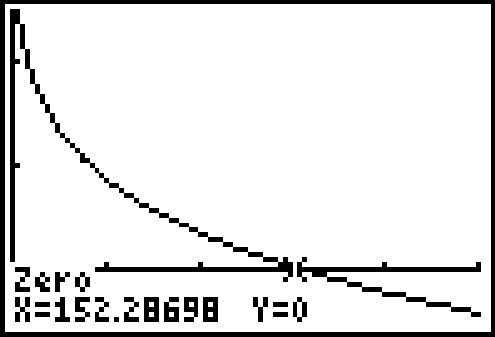
\includegraphics[width=1.75in]{./FurtherGraphics/WINDCHILL.jpg}}


\end{enumerate}

\item $9.8 \left(\dfrac{1}{4\pi}\right)^{2} \approx 0.062$ meters or $6.2$ centimeters

\item \begin{enumerate}

\item First rewrite the model as $P = 1.23x^{\frac{2}{5}}y^{\frac{3}{5}}$.  Then $300 = 1.23x^{\frac{2}{5}}y^{\frac{3}{5}}$ yields $y = \left( \dfrac{300}{1.23x^{\frac{2}{5}}} \right)^{\frac{5}{3}}$.  If $x = 100$ then $y \approx 441.93687$.

\end{enumerate}

\item \begin{enumerate}

\item $[0, c)$

\item $~$

\begin{tabular}{ll} 
$m(.1c) = \dfrac{m_{r}}{\sqrt{.99}} \approx 1.005m_{r}$ & $m(.5c) = \dfrac{m_{r}}{\sqrt{.75}} \approx 1.155m_{r}$\\ \smallskip

$m(.9c) = \dfrac{m_{r}}{\sqrt{.19}} \approx 2.294m_{r}$ & $m(.999c) = \dfrac{m_{r}}{\sqrt{.0.001999}} \approx 22.366m_{r}$ \\ \end{tabular}


\item As $x \rightarrow c^{-}, \, m(x) \rightarrow \infty$

\item If the object is traveling no faster than approximately $0.99995$ times the speed of light, then its observed mass will be no greater than $100m_{r}$.

\end{enumerate}


\item $k^{-1}(x) = \dfrac{x}{\sqrt{x^{2} - 4}}$

\item \begin{enumerate}

\item  $y = \frac{1}{3}x^{3/2} - \sqrt{x} + \frac{2}{3}$.  The point $\left(0,\frac{2}{3}\right)$ is when Fritzy's path crosses Chewbacca's path - in other words, where Fritzy catches Chewbacca.

\item $y = \frac{1}{6}x^3+\frac{1}{2x} - \frac{2}{3}$.  Using the techniques from Chapter \ref{Rationals}, we find as $x \rightarrow 0^{+}$, $y \rightarrow \infty$ which means, in this case, Fritzy's pursuit never ends;  he never catches Chewbacca. This makes sense since Chewbacca has a head start and is running faster than Fritzy.

\begin{center}

\begin{tabular}{cc}

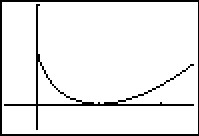
\includegraphics[width=2in]{./FurtherGraphics/PURSUIT01.jpg} & \hspace{1in} 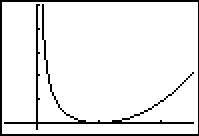
\includegraphics[width=2in]{./FurtherGraphics/PURSUIT02.jpg}  \\

$y = \frac{1}{3}x^{3/2} - \sqrt{x} + \frac{2}{3}$ & \hspace{1in} $y = \frac{1}{6}x^3+\frac{1}{2x} - \frac{2}{3}$ \\

\end{tabular}

\end{center}

\end{enumerate}


\end{enumerate}

\closegraphsfile